\documentclass[letter]{article}

\usepackage[dvipsnames]{xcolor}
\usepackage[T1]{fontenc}
\usepackage[utf8]{inputenc}
\usepackage{lmodern}

\usepackage[english]{babel}
\usepackage{csquotes}
\usepackage{multirow}
\usepackage{amssymb,amsmath,amsfonts} % nice math rendering

\usepackage{caption}
\usepackage{subcaption}
\usepackage{fancyhdr}
\usepackage{booktabs}
\usepackage{textcomp}
\usepackage{gensymb}
\usepackage{graphicx}
\usepackage{todonotes}
\usepackage{floatrow}
\usepackage{hyperref}
\usepackage{lastpage}

\usepackage{braket} % needed for \Set
\usepackage{algorithm}
\usepackage[noend]{algpseudocode}
\DeclareMathOperator*{\argmax}{arg\,max}

\graphicspath{ {./images/} }

\usepackage[margin=0.8in]{geometry}

\usepackage[notes,backend=biber]{biblatex-chicago}
\bibliography{sample}

\begin{document}
\title{MDPs and RL - CS 4641}
\author{Omar Shaikh}
\maketitle

\begin{abstract}
    In this report, I explore three RL methods of interest. The first two are Policy and Value iteration, both rooted in Dynamic Programming Techniques. I also explore the relationship between living penalties and discounts for DL approaches. The last method, Q-learning, utilizes TD learning unlike the first two. I compare and contrast both value and policy iteration in two MDPs; finally, I conclude with an exploration of Q-learning strategies and a general comparative analysis.
\end{abstract}

\section{Markov Decision Processes}

A state $S_t$ is Markov if and only if
\begin{equation}
\mathbb{P}[S_{t+1}|S_t] = \mathbb{P}[S_{t+1}|S_1, ... , S_t]
\end{equation}
A future is independent of the past given the present. We use state transition matrix $P$ to define transition probabilities from all states $s$ to all successor states $s'$\autocite{Sutton:1998:IRL:551283}
\begin{equation}
P_{ss'}=\mathbb{P}[S_{t+1}=s'|S_t=s]
\end{equation}
The following MDP follows Markov assumption.

\subsection{Frozen Cliff MDP}

The general MDP used in this project is a slightly altered version of the Frozen Cliff MDP taken from OpenAI's gym\autocite{1606.01540}.  

\begin{quote}
    Winter is here. You and your friends were tossing around a frisbee at the park
    when you made a wild throw that left the frisbee out in the middle of the lake.
    The water is mostly frozen, but there are a few holes where the ice has melted.
    If you step into one of those holes, you'll fall into the freezing water.
    At this time, there's an international frisbee shortage, so it's absolutely imperative that
    you navigate across the lake and retrieve the disc.
    However, the ice is slippery, so you won't always move in the direction you intend.
    The surface is described using a grid like the following (\ref{fig1:smallmdp})

    S : starting point, safe\\
    F : frozen surface, safe\\
    H : hole, fall to your doom\\
    G : goal, where the frisbee is located

    The episode ends when you reach the goal or fall in a hole.
    You receive a reward of 1 if you reach the goal, and zero otherwise.
\end{quote}
The slight alteration comes in the form of a small negative living reward, to enforce a horizon on the MDP. If the agent doesn't fall into a hole, but doesn't reach it's goal-state, it receives a small pre-defined penalty. My attached code was stolen mostly from the cited GitHub repository \autocite{cmaron-github}.

\subsection{Problem Instances and Interest}
The following two frozen lakes highlight our MDPs. For my environments, I added a custom transition matrix defined in \ref{eq:mdptransition}, where the intended action $x$ is parameterized by probability $p$. Whenever p is referenced from now, assume I'm referring to this transition setup. Think of increasing p as increasing stochasticity in the environment.

For both my MDPs (\ref{fig1:largemdp} and \ref{fig1:smallmdp}) I have a single goal state in the bottom right corner. However, with the larger MDP, there are more (terminal) states which will require more time for our RL algorithms to converge. Furthermore, there are several paths we can see in the large MDP, and the solution is somewhat vague. With the small MDP, the optimal policy can be eyeballed given parameters. 

\begin{figure}
    \centering
    \begin{subfigure}{.5\textwidth}
        \centering
        \texttt{\textcolor{blue}{S}FFF}\\
        \texttt{F\textcolor{red}{H}F\textcolor{red}{H}}\\
        \texttt{FFF\textcolor{red}{H}}\\
        \texttt{HFF\textcolor{green}{G}}
        \caption{Small MDP (4x4)}
        \label{fig1:smallmdp}
      \end{subfigure}%
    \begin{subfigure}{.5\textwidth}
      \centering
      \centering
      \texttt{\textcolor{blue}{S}FFFFFF\textcolor{red}{H}\textcolor{red}{H}\textcolor{red}{H}FFFFFFFFFF}\\
      \texttt{FFFFFFFFFFFFFFFF\textcolor{red}{H}\textcolor{red}{H}FF}\\
      \texttt{FFF\textcolor{red}{H}FFFFFFF\textcolor{red}{H}\textcolor{red}{H}FFFFFFF}\\
      \texttt{FFFFF\textcolor{red}{H}FFFFFFFFFF\textcolor{red}{H}\textcolor{red}{H}FF}\\
      \texttt{FFFFF\textcolor{red}{H}FFFFFFFFFF\textcolor{red}{H}\textcolor{red}{H}FF}\\
      \texttt{FFFFF\textcolor{red}{H}FFFFFFFFFF\textcolor{red}{H}\textcolor{red}{H}FF}\\
      \texttt{FFFFFFFF\textcolor{red}{H}FFFFFFF\textcolor{red}{H}\textcolor{red}{H}FF}\\
      \texttt{FFFFF\textcolor{red}{H}FFFF\textcolor{red}{H}\textcolor{red}{H}FFFF\textcolor{red}{H}\textcolor{red}{H}FF}\\
      \texttt{FFFFF\textcolor{red}{H}FFFFFFFFFF\textcolor{red}{H}\textcolor{red}{H}FF}\\
      \texttt{FFFFF\textcolor{red}{H}FFFFFFFFFF\textcolor{red}{H}\textcolor{red}{H}FF}\\
      \texttt{FFFFFFFFFFF\textcolor{red}{H}\textcolor{red}{H}\textcolor{red}{H}\textcolor{red}{H}\textcolor{red}{H}\textcolor{red}{H}\textcolor{red}{H}FF}\\
      \texttt{\textcolor{red}{H}\textcolor{red}{H}\textcolor{red}{H}\textcolor{red}{H}F\textcolor{red}{H}FFFFFFFFFF\textcolor{red}{H}\textcolor{red}{H}FF}\\
      \texttt{FFFFF\textcolor{red}{H}FFFF\textcolor{red}{H}\textcolor{red}{H}\textcolor{red}{H}FFF\textcolor{red}{H}\textcolor{red}{H}FF}\\
      \texttt{FFFFFFFFFFFFFFFF\textcolor{red}{H}\textcolor{red}{H}FF}\\
      \texttt{FFFFF\textcolor{red}{H}FFFFFF\textcolor{red}{H}FFF\textcolor{red}{H}\textcolor{red}{H}FF}\\
      \texttt{FFFFF\textcolor{red}{H}FFFFFFFFFF\textcolor{red}{H}\textcolor{red}{H}FF}\\
      \texttt{FFFFFFFFFFF\textcolor{red}{H}FFFFFFFF}\\
      \texttt{F\textcolor{red}{H}\textcolor{red}{H}FFF\textcolor{red}{H}FFFF\textcolor{red}{H}FFFFF\textcolor{red}{H}FF}\\
      \texttt{F\textcolor{red}{H}\textcolor{red}{H}F\textcolor{red}{H}F\textcolor{red}{H}FFFFFFFFFFFFF}\\
      \texttt{FFF\textcolor{red}{H}FFFFF\textcolor{red}{H}FFFF\textcolor{red}{H}\textcolor{red}{H}F\textcolor{red}{H}F\textcolor{green}{G}}      
      \caption{Large MDP (20x20)}
      \label{fig1:largemdp}
    \end{subfigure}
    \caption{Frozen Cliff Environments}
\end{figure}
    

\begin{equation}
    \label{eq:mdptransition}
    S_{t+1}(x) = 
    \begin{cases}
        x,& \text{with probability } 1-p\\
        rotate(x, 90\degree),              & \text{with probability } \frac{p}{2}\\
        rotate(x, -90\degree),              & \text{with probability } \frac{p}{2}
    \end{cases}
\end{equation}

Note that this MDP is quite similar to GridWorld detailed in literature, except that the transition matrix doesn't account for the agent accidentally moving backward (we assume that the person looking for the frisbee won't mess up too badly). Because of this, we can directly rely on prior observations from GridWorld (due to the research attention this problem has received), while exploring a slightly different MDP formulation.

\section{Computer Specifications}
The computer used to train and test has an i7-7700HQ (clock speeds @ 3.8 GHZ), 32 GB of RAM, and an Nvidia GTX 1070 with 8 GB of VRAM. Whenever it was possible, I used all CPU cores. Runtimes of algorithms should be considered in context of these specifications.
\section{Model Based Learners \& Dynamic Programming}
The following subsections cover Learning Algorithms that rely on Bellman's equations and Dynamic Programming techniques.

In the case of value iteration, the optimal value for each state is calculated, where the value is defined as the sum of maximum reward following the best policy. In the case of value iteration, the best policy can be defined by greedily picking a route of the maximum value at each state. Note that we are not finished until each value for every state has converged (see algorithm \ref{alg:value-iteration}).

With policy iteration, however, we pick a random initial policy and solve a set of linear equations to justify actions at every step in our policy. When our actions stop changing (e.g all states have been "justified") we converge at our final policy. Note, however, that each iteration takes more effort on the part of policy iteration when compared to value iteration due to solving this system of equations (see algorithm \ref{alg:policy-iteration}). 

For both problems, I wanted to test a small negative punishment and a discounting factor to see if, in my worlds, they serve the same purpose. Discounting appears to serve a geometric purpose -- going further away from the goal decreases the rewards of the goal geometrically, which (I hypothesize) establishes an event horizon. The same can be said for a small negative penalty. However, in the case of the penalty, our reward is an arithmetic progression. 

The aforementioned MDPs, therefore, are tested on two cases:

\begin{itemize}
    \item Case I (living penalty): No discounting factor with a negative living reward of -.1
    \item Case II (discounted): A discounting reward of .9, with no negative living reward.
\end{itemize}

To compare policies, I decided to analyze the case where $p=1/5$. this was chosen somewhat arbitrarily (I wanted to see a slightly cautious agent at work -- not a bumbling fool or a perfectionist).

\begin{algorithm}[H]
    \begin{algorithmic}
    \Require
    \Statex States $\mathcal{X} = \{1, \dots, n_x\}$
    \Statex Actions $\mathcal{A} = \{1, \dots, n_a\},\qquad A: \mathcal{X} \Rightarrow \mathcal{A}$
    \Statex Cost function $g: \mathcal{X} \times \mathcal{A} \rightarrow \mathbb{R}$
    \Statex Transition probabilities $f_{xy}(a) = \mathbb{P}(y | x, a)$
    \Statex Discounting factor $\alpha \in (0, 1)$, typically $\alpha = 0.9$
    \Procedure{ValueIteration}{$\mathcal{X}$, $A$, $g$, $f$, $\alpha$}
        \State Initialize $J, J': \mathcal{X} \rightarrow \mathbb{R}_0^+$ arbitrarily
        \While{$J$ is not converged}
            \State $J' \gets J$
            \For{$x \in \mathcal{X}$}
                \For{$a \in A(x)$}
                    \State $Q(x, a) \gets g(x, a) + \alpha \sum_{j=1}^{n_x} f_{xj}(a) \cdot J'(j)$
                \EndFor
            \EndFor
            \For{$x \in \mathcal{X}$}
                \State $J(x) \gets \min_a \{Q(x, a)\}$
            \EndFor
        \EndWhile
        \Return $J$
    \EndProcedure
    \end{algorithmic}
\caption{Value Iteration\autocite{Sutton:1998:IRL:551283}: Learn function $J: \mathcal{X} \rightarrow \mathbb{R}$}
\label{alg:value-iteration}
\end{algorithm}

\begin{algorithm}[H]
    \begin{algorithmic}
    \Require
    \Statex States $\mathcal{X} = \{1, \dots, n_x\}$
    \Statex Actions $\mathcal{A} = \{1, \dots, n_a\},\qquad A: \mathcal{X} \Rightarrow \mathcal{A}$
    \Statex Cost function $g: \mathcal{X} \times \mathcal{A} \rightarrow \mathbb{R}$
    \Statex Transition probabilities $f$, $F$
    \Statex $\alpha \in (0, 1)$
    \Procedure{PolicyIteration}{$\mathcal{X}$, $A$, $g$, $f$, $F$, $\alpha$}
        \State Initialize $\pi$ arbitrarily
        \While{$\pi$ is not converged}
            \State $J \gets$ solve system of linear equations $(I - \alpha \cdot F(\pi)) \cdot J = g(\pi)$

            \For{$x \in \mathcal{X}$}
                \For{$a \in A(x)$}
                    \State $Q(x, a) \gets g(x, a) + \alpha \sum_{j=1}^{n_x} f_{xj}(a) \cdot J(j)$
                \EndFor
            \EndFor
            \For{$x \in \mathcal{X}$}
                \State $\pi(x) \gets \arg \min_a \{Q(x, a)\}$
            \EndFor
        \EndWhile
        \Return $\pi$
    \EndProcedure
    \end{algorithmic}
\caption{Policy Iteration\autocite{Sutton:1998:IRL:551283}: Learning a policy $\pi: \mathcal{X} \rightarrow \mathcal{A}$}
\label{alg:policy-iteration}
\end{algorithm}

\begin{figure}[]
    \centering
    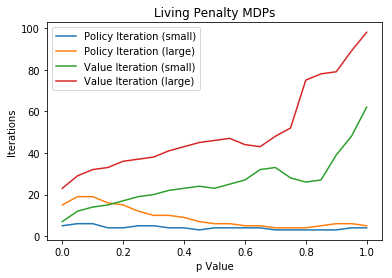
\includegraphics[width=.4\linewidth]{penalty_iterations.png}
    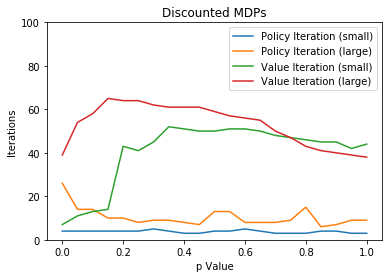
\includegraphics[width=.4\linewidth]{discounted_iterations.png}
    \caption{Iterations to converge w.r.t p Value on Case I (left) and Case II (right) MDPs}
    \label{iterationsFig}
\end{figure}


\begin{figure}[]
    \centering
    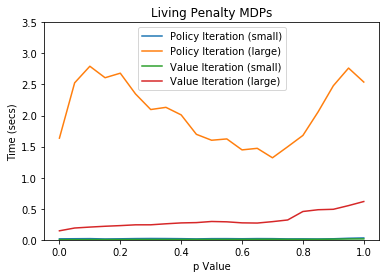
\includegraphics[width=.4\linewidth]{penalty_time.png}
    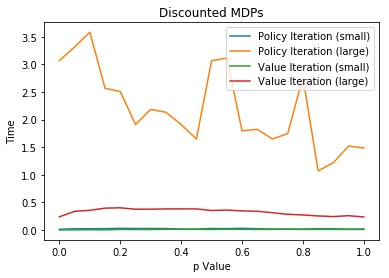
\includegraphics[width=.4\linewidth]{discounted_time.png}
    \caption{Time to converge w.r.t p Value on Case I (left) and Case II (right) MDPs}
    \label{timeFig}
\end{figure}

\subsection{Problem \ref{fig1:smallmdp} - Small MDP}
In the case of the smaller MDP, the difference in evaluation time to convergence across all values of p is negligible, as seen in Fig \ref{timeFig}. However, in terms of iterations, value iteration takes far more steps for all values of p when compared to policy iteration (Fig \ref{iterationsFig}). All of these observations apply to both Case I and Case II MDPs, and will be discussed in comparative analysis.

In terms of generated policy, VI and PI converged, and to the same result -- this also will be revisited in the comparative analysis (hence only one figure for both, Fig \ref{smallPolicies}).

\subsection{Problem \ref{fig1:largemdp} - Big MDP}

In the case of the large MDPs, the disparity between VI and PI becomes more apparent. With the Case I and Case II MDPs, VI takes more iterations than PI again \ref{iterationsFig}, but PI takes more time than PI \ref{timeFig}.

In terms of generated policy, again VI and PI converged to the same result -- this will be revisited in the comparative analysis (hence only one figure for both, Fig \ref{largePolicies}).


\begin{figure}[]
    \centering
    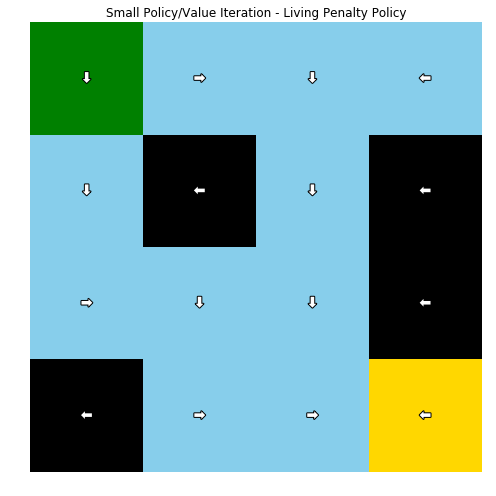
\includegraphics[width=.4\linewidth]{smallLivingPenaltyPolicy.png}
    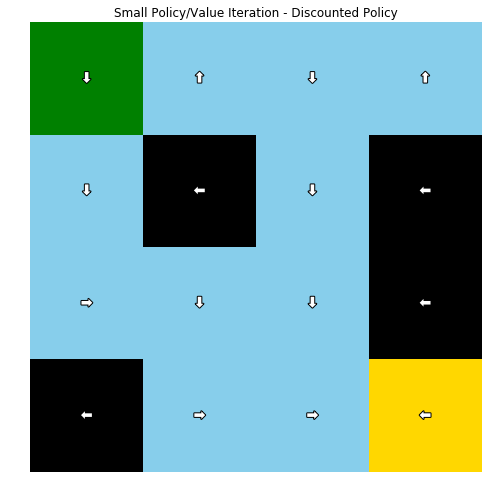
\includegraphics[width=.4\linewidth]{smallDiscountedPolicy.png}
    \caption{VI and PI Policy for Case I (left), Case II (right) when p = .2 on small MDP}
    \label{smallPolicies}
\end{figure}

\begin{figure}[]
    \centering
    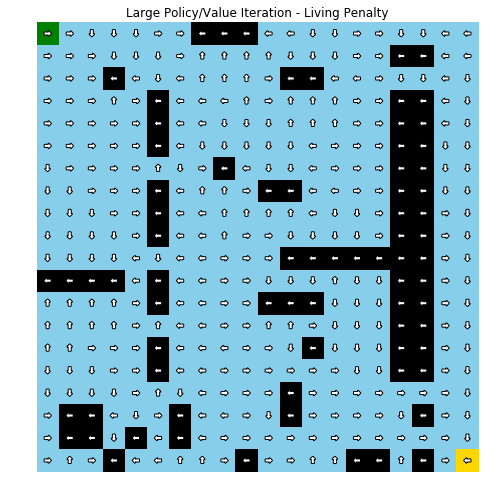
\includegraphics[width=.4\linewidth]{largeLivingPenaltyPolicy.png}
    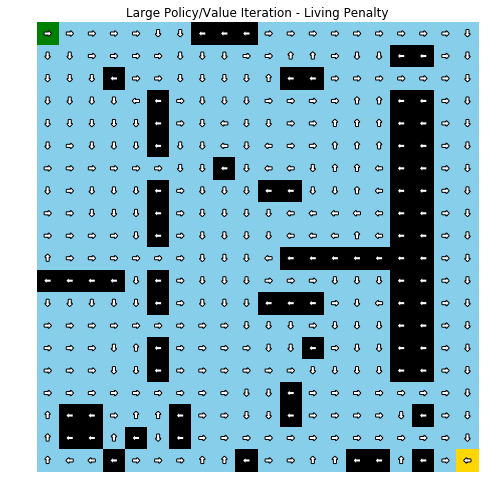
\includegraphics[width=.4\linewidth]{largeDiscountedPolicy.png}
    \caption{VI and PI Policy for Case I (left), Case II (right) when p = .2 on Large MDP}
    \label{largePolicies}
\end{figure}


\subsection{Comparative Analysis}

\subsubsection{Similar Policies and Increased Iterations}
Unsurprisingly, the policies for value and policy iteration were the same. This should usually be expected, because value iteration is a "stricter" policy iteration. While value iteration waits for the individual values to converge, policy stops iterating when the greedily picked individual steps stop changing. 

This might lead one to think that policy iteration should always be faster; however, in the case of policy, we're solving a system of linear equations across all actions for each iteration of the algorithm (observe the while not converged condition in \ref{alg:value-iteration} and \ref{alg:policy-iteration}). This is why, despite the lower iterations for VI, our PI takes noticeably longer in terms of evaluation time for all values of p.

There does exist a difference in final policies when comparing Case I and Case II MDPs. 

With the small MDP policies (Fig \ref{smallPolicies}), sometimes the discounted policy doesn't head toward the goal state, taking the safer route early on. This is probably because the hole is close to the start state, so its punishment hasn't been discounted significantly enough for the agent to consider the "riskier" route. The living penalty, however, takes more risky steps since the penalty doesn't decrease as time increases.

The difference between Case I and II is more apparent when the MDP state space is larger. For Case I MDPs, the sum of living penalties is too high to consider getting to the goal, so the new goal becomes suicide. Although the discounted Case II MDPs will have a low goal reward, it still will be possible to achieve this reward, which encourages the agent to go for it.

My conclusion is that, in the case of a larger state space, a discount is more standardized than a negative penalty, especially if the optimal outcome is the agent achieving said goal. Sure, one could play with the size of the goal reward, but in a more complex MDP estimating this reward may be difficult.

\subsubsection{Size and Performance}
For both our problems, I noticed that PI takes takes significantly more time to converge when the state space increases when compared to VI. This is the case for both MDP variants I tested. Even though VI's iterations increase as the state space increases, it's evaluation time doesn't take as a big a hit as PI. 

Again, the reasoning behind this lies in the prior subsection (3.3.1). Large state spaces may suffer with PI because we need to solve a complex system of linear equations. In some cases (i.e mine), VI will converge to individual values quicker, but will require more iterations.

The tradeoff we need to observe is time v iterations. For PI, each iteration requires more compute power, whereas with VI, we need more iterations w/ less compute power.

\subsubsection{Observing $p$ value and MDP Cases}
Our relationship between iterations and value of p for the large MDPs also appears interesting. As we increase our p value for the Case I (living penalty) MDPs, our iterations increase for VI. Oddly, for the discounted MDPs, they appear to fall as p increases. 

I suspect that the early suicidal tendencies of the Case I living penalty MDPs makes increasing p a difficulty. As p increases, we're increasing stochasticity in the environment, which makes it harder for the Case I agent to decide where to terminate itself. Getting to the goal state is out of the question entirely (as discussed in subsection 3.3.1), as the living penalty overwhelms the final +1 goal reward.

With Case II Large MDPs, there's a decrease in iterations compared to p. I suspect that the discounting ensures that the MDP tries to find the shortest path to the goal while not losing faith (due to the living penalty overwhelming the reward). The losing faith aspect of the living reward.

\begin{figure}[]
    \centering
    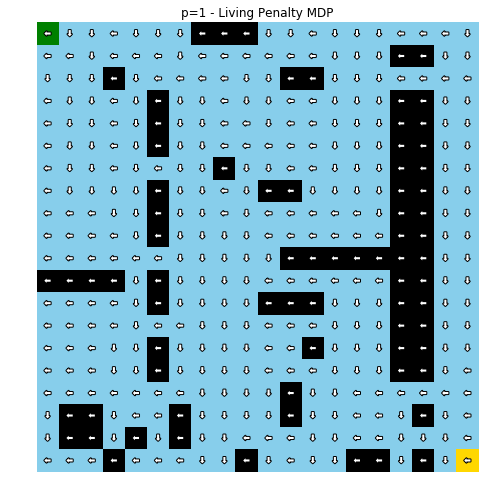
\includegraphics[width=.4\linewidth]{p1penalty.png}
    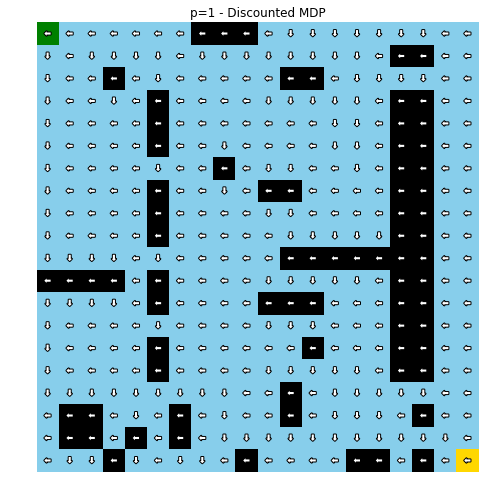
\includegraphics[width=.4\linewidth]{p1discounted.png}
    \caption{Case I (left) and Case II (right) MDPs when p=1}
    \label{p1fig}
\end{figure}

Looking at the the large MDPs when p=1 is very interesting. The discounted MDP appears to have learned that its intended actions always go wrong, and never goes in the direction it should go in (since the probability of the intended action occurring is 0). In fact, it heads towards the holes because it knows with certainty that it will not fall into them (Fig \ref{p1fig}, right)!

The living penalty MDP, however, will commit wrong actions closer to the goal (in hopes that it will fall in) and correct (hole avoiding) actions father away (Fig \ref{p1fig}, left). These MDPs are sorta like inception MDPs, in that they learn to manipulate the deceptive world they're in (I'm still in shock this is actually wild).

\section{TD (Q) Learning}
TD Learning techniques are significantly different from DP techniques in that a policy is generated from a sequence of steps fed to the algorithm. A policy isn't generated through exploring every possible state's policy -- instead, sequences of states dictate how and what policy is generated.

One example of such an algorithm is Q-learning (Algorithm \ref{alg:q-learning}). For our sequence exploration strategy, I used the epsilon greedy strategy. Epsilon-greedy works like simulated annealing, exploring sequences at rate epsilon and picking the greedy route otherwise. Different strategies were explored by using different values of epsilon. For my experiments, I looked at the effects of two parameters on Q-learning (p and epsilon) and total reward and the evaluation time. 

Iterations for Q-Learning were fixed @ a max of 1,000 and 5,000 episodes for control on the small and large MDPs respectively. Averages of 20 trials were taken in some cases to avoid variance due to randomization. Q-learners were run till convergence. Learner performance was measured by the sum of episode scores for each learning iteration. Problem instances from subsection 1.2 will be reused; however, this subsection will only focus on Case II MDPs for the sake of brevity.
 
\begin{algorithm}[H]
    \begin{algorithmic}
    \Require
    \Statex States $\mathcal{X} = \{1, \dots, n_x\}$
    \Statex Actions $\mathcal{A} = \{1, \dots, n_a\},\qquad A: \mathcal{X} \Rightarrow \mathcal{A}$
    \Statex Reward function $R: \mathcal{X} \times \mathcal{A} \rightarrow \mathbb{R}$
    \Statex Black-box (probabilistic) transition function $T: \mathcal{X} \times \mathcal{A} \rightarrow \mathcal{X}$
    \Statex Learning rate $\alpha \in [0, 1]$, typically $\alpha = 0.1$
    \Statex Discounting factor $\gamma \in [0, 1]$
    \Procedure{QLearning}{$\mathcal{X}$, $A$, $R$, $T$, $\alpha$, $\gamma$}
        \State Initialize $Q: \mathcal{X} \times \mathcal{A} \rightarrow \mathbb{R}$ arbitrarily
        \While{$Q$ is not converged}
            \State Start in state $s \in \mathcal{X}$
            \While{$s$ is not terminal}
                \State Calculate $\pi$ according to Q and exploration strategy (e.g. $\pi(x) \gets \argmax_{a} Q(x, a)$)
                \State $a \gets \pi(s)$
                \State $r \gets R(s, a)$ \Comment{Receive the reward}
                \State $s' \gets T(s, a)$ \Comment{Receive the new state}
                \State $Q(s', a) \gets (1 - \alpha) \cdot Q(s, a) + \alpha \cdot (r + \gamma \cdot \max_{a'} Q(s', a'))$
                \State $s \gets s'$
            \EndWhile
        \EndWhile
        \Return $Q$
    \EndProcedure
    \end{algorithmic}
\caption{$Q$-learning: Learn function $Q: \mathcal{X} \times \mathcal{A} \rightarrow \mathbb{R}$}
\label{alg:q-learning}
\end{algorithm}

\begin{figure}[]
    \centering
    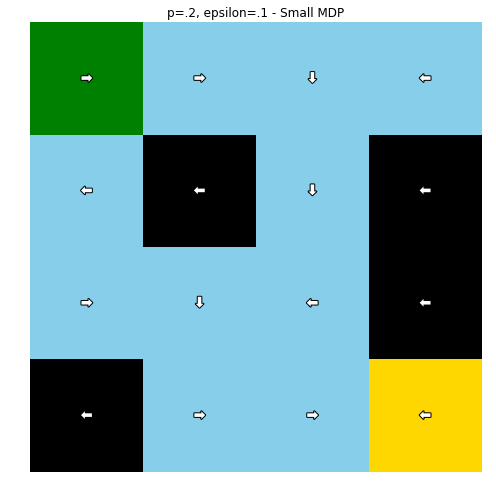
\includegraphics[width=.4\linewidth]{qlearn_small_ol.png}
    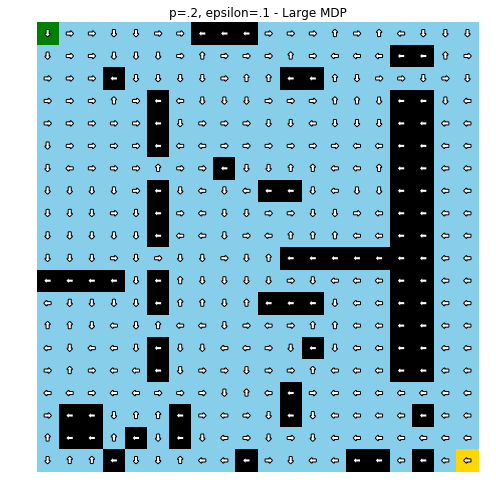
\includegraphics[width=.4\linewidth]{qlearn_large_ol.png}
    \caption{Misc Q-learning Optimal Policies for Small (left) and Large (right) Instances.}
    \label{polq}
\end{figure}

\subsection{Effects of epsilon and p on Reward}
\begin{figure}[]
    \centering
    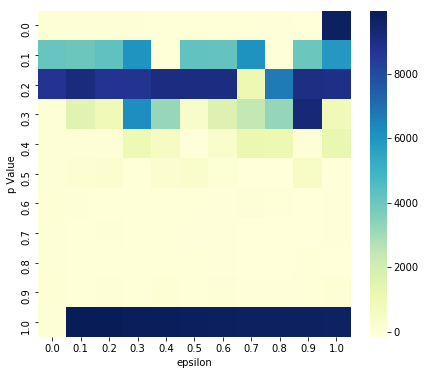
\includegraphics[width=.4\linewidth]{small_ep_p.png}
    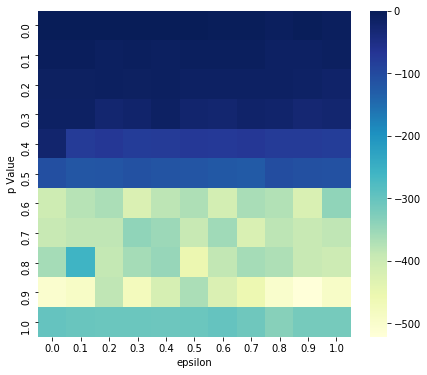
\includegraphics[width=.4\linewidth]{large_ep_p.png}
    \caption{Sum of Episode Rewards for Small (left) and Large (right) Problem given p and epsilon.}
    \label{epsilon_p}
\end{figure}
\subsubsection{Problem \ref{fig1:smallmdp} - Small MDP}
Epsilon doesn't seem to have much of an effect on the rewards for our small MDP (see Fig \ref{epsilon_p}), possibly because not much exploration needs to occur for us to find the optimal path -- we can exhaust most of the search space even if we rarely explore and mostly exploit. P, however, does have an effect. Increasing it adds more uncertainty to our environment. Because we limited the number of iterations in our environment, increasing P ends up reducing our Q-learning scores. Oddly, with $p=1$, we also converge to an optimal solution. This occurs because the Q-learner quickly learns that the reverse of its world is true, and exploits it (similar to the phenomenon we saw in FIg \ref{p1fig})

The optimal policy is a little alarming though -- it looks like the same assumption I built regarding reward from the model based learners don't apply to Q-learners. \textbf{One state far away from the goal, for example, avoids the goal state entirely}(see Fig \ref{polq}). Generated sequences probably take longer paths to our goal state, so by the time they arrive, the goal state is worth nothing. Increasing the reward of the goal state fixes this problem. 

\subsubsection{Problem \ref{fig1:largemdp} - Big MDP}
Unlike the small MDP, changing epsilon changes our Q-learning rewards (up to a point, see Fig \ref{epsilon_p}). Because we have more obstructions, exploring to find an optimal path becomes necessary. P also has the same effect as with the above subsection, yet worse. Because we're adding more uncertainty to a larger map, the uncertainty "propagates," affecting our final score. Epsilon didn't have the effect I wanted it to, but this may be due to the limited number of iterations.

Also regarding the limit on iterations: our policy doesn't come close to the optimal state. Some of the nonsensical moves in the large MDP policy also appear to stem from the discount factor \ref{polq}. Future work could clarify the relationship between discount factors and Q-learning.

\subsection{Effects of epsilon on evaluation time}
There is an odd outlier for the small MDP at $p=1$ -- it looks like the initial policy for the Q-learner is very close to the optimal policy, so no steps are required. 

From Figure \ref{epTime}, we can see that epsilon has a serious impact on evaluation time. From the first half of epsilons domain, it appears that the evaluation time follows an exponential trend. This makes sense, since by increasing epsilon we're performing more computationally expensive exploration (due to epsilon greedy following Boltzmann's distribution). In practical cases, especially if the environment is constrained, someones this tradeoff should be looked at more carefully.

\begin{figure}[]
    \centering
    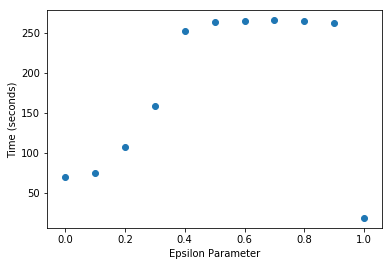
\includegraphics[width=.4\linewidth]{epsilon_time_small.png}
    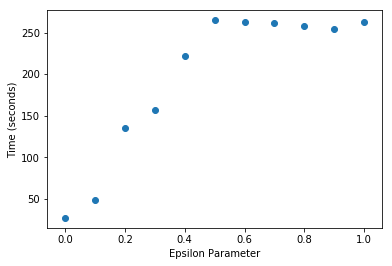
\includegraphics[width=.4\linewidth]{epsilon_time_large.png}
    \caption{Average Convergence Time for Small (left) and Large (right) MDP given epsilon}
    \label{epTime}
\end{figure}
\subsection{Comparison between Q-Learning and Model Based Learners}
\subsubsection{Policies}
On both maps, Q-learning produced policies (see Fig \ref{polq}, \ref{largePolicies}, \ref{smallPolicies}) that were not as good as the ones produced by model based learners, and not even close when the size of the problem increased. This should be expected since Q-learners don't have nearly as much information about the environment as the model based learner (i.e no transition model, no rewards, etc). Also, sometimes the intermediate policies have odd behaviors (going to dangerous/useless places in the environment).
\subsubsection{Runtime}
In case of runtimes, Q-learning dwarfs Model-Based learners (see Fig \ref{epTime} and Fig \ref{timeFig}). The tradeoff here is information v time. Q learners need more time to learn the underlying transition probabilities from the sample sequences it receives. Model based learners can get converging towards an optimal policy instantly, instead of learning the environment through trial and error. In fact, the entire algorithm (\ref{alg:q-learning}) hinges on generating new (s, a, s', r) tuples to explore the environment and come to an optimal policy.
\subsubsection{Effect of p}
Q-learning scores were heavily dependent on the value of p (as seen in Fig \ref{epsilon_p}), moreso than their model based counterparts. Because the transition models are baked into the Q-table, the Q-learner takes more time (depending on our choice of P) to learn the model. Because we fixed our Q-learner to a constant number of iterations, the relationship is fairly clear.

\section{Conclusion A.K.A "which one should I use?"}
In the case that we do have a transition model and an approachable state space, using a Model Based Learner makes sense. There's no point in wasting compute to learn the environnement when we already have an explicit description. If our state space is extraordinary large, value iteration may be faster than policy iteration -- otherwise, PI is a better choice if utility at every state isn't important.

If we don't have an explicit transition model for our environment, then using a model-based learner is simply not an option. Q-learning solves this problem, along with experimenting and using domain-knowledge to pick a good epsilon model for exploration/exploitation.

\printbibliography

\end{document}